% 
%
\newgeometry{top=2cm, bottom=1cm, left=1cm, right=1cm,
               marginparsep=0cm, marginpar=0pt}
\makeatletter
\cxset{kroll scale/.store in = \scalekroll@cx,
       kroll left column width/.store in = \krollleftcolumnwidth@cx,
       kroll imagei/.store in = \krollimagei@cx,
       kroll imagei caption/.store in = \krollimageicaption@cx,
       kroll imageii/.store in = \krollimageii@cx,
       kroll imageii caption/.store in = \krollimageiicaption@cx,
       kroll left header/.store in = \krollleftheader@cx,
       kroll header/.store in = \krollheader@cx}

\cxset{kroll scale = 1,
       kroll left column width = {\dimexpr\textwidth-.4\textwidth\relax},
       kroll left header =,
       kroll imagei = bache-01,
       kroll imagei caption ={\begin{multicols}{2}\lorem\end{multicols}},
       kroll imageii = nudeback,
       kroll imageii caption = {NUDE  BACK  SHOWS   A  DANCER  WHOSE  BACK  SAYS  KROLL,  HAS  BEAUTIFUL  PLANES},
       kroll header = \scalebox{.97}{THE DEAN OF US NUDE-PAINTERS}
    }
\newenvironment{kroll}{%
\parindent0pt
\renewenvironment{leftcolumn}{%
   \minipage[t]{\krollleftcolumnwidth@cx}%
\leavevmode   
  }{\endminipage}\hspace*{0cm}%

 \renewenvironment{rightcolumn}{%
   \minipage[t][\textheight-20pt][t]{.37\textwidth}%
   \mbox{}%
  }{\endminipage}\hspace*{0cm}% 

\begin{minipage}[t][\textheight][t]{\scalekroll@cx\textwidth}%
{\hrule\vbox to 0pt{\rule{1pt}{\textheight}}
 \leavevmode\Large\bfseries\sffamily JULES BACHE GIVES HIS \$20,000,000 ART COLLECTION TO NEW YORK\par}%
\begin{leftcolumn}%
\mbox{}%ncessesary to line on top
\par\leavevmode\includegraphics[width=\linewidth]{\krollimagei@cx}\par
\krollimageicaption@cx%
\end{leftcolumn}\hfill%
\begin{rightcolumn}%
  \leavevmode
 }
{\end{rightcolumn}%
\end{minipage}} 
\begin{kroll}
\begin{wrapfigure}{l}{3.2cm}
  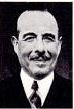
\includegraphics[width=3cm]{bache-02}
    %\caption{\footnotesize Wrapped figures}
\end{wrapfigure}
This layout has a dominant left column image. It is important to
ensure that the image has an aspect ratio to suit. Unfortunately
it is very difficult to crop and scale an image via \tex so a bit
of experimentation is appropriate.

It is also important to ensure that you add an adequate amount
of text during editing, otherwise the layout will not look very good. The right
column has two images (it really looks better when it has two images rather than
one and the bottom image is really a filler, if you have more or less
text you may have to go back and crop the image to suit. Any extra space on the right column is used as glue.

\vfill
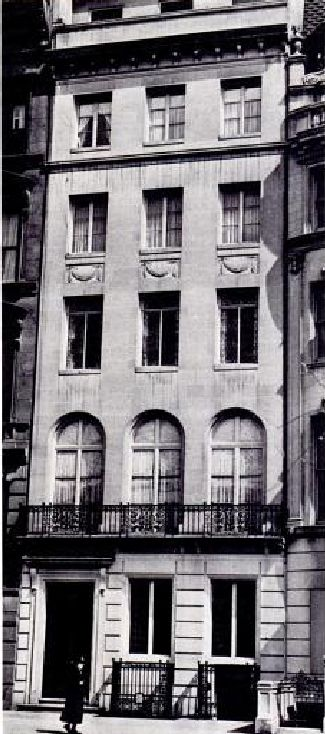
\includegraphics[width=\linewidth]{bache-03}
\end{kroll}



\restoregeometry